% Uncomment this to make slides with overlays:
\documentclass[slides]{beamer}

% Uncomment these (but comment the above \documentclass line) to make handouts:
%\documentclass[handout]{beamer}

% Uncomment these to have more than one slide per page
%\usepackage{pgfpages}
%\pgfpagesuselayout{2 on 1}[border shrink=5mm]
%\pgfpageslogicalpageoptions{1}{border code=\pgfusepath{stroke}}
%\pgfpageslogicalpageoptions{2}{border code=\pgfusepath{stroke}}

\usepackage[]{graphicx, color, hyperref}

\mode<presentation>
{
	%\usetheme[secheader]{Boadilla}
	%\usecolortheme[rgb={.835, .102,.169}]{structure}  
	\usetheme[width= 0cm]{Goettingen}
	%\setbeamercovered{transparent}
}
\setbeamertemplate{navigation symbols}{}
\setbeamertemplate{footline}[frame number]

\definecolor{blue2}{rgb}{0.278,0.278,0.729} 
\newcommand{\blue}[1]{\textcolor{blue2}{#1}}
\newcommand{\white}[1]{\textcolor{white}{#1}}
\newcommand{\red}[1]{\textcolor{red}{#1}}
\newcommand{\xbar}{\overline{x}}
\newcommand{\ybar}{\overline{y}}
\newcommand{\phat}{\widehat{p}}
\newcommand{\prob}{\mbox{Pr}}
\newcommand{\E}{\mathbb{E}}
\newcommand{\Var}{\mbox{Var}}
\newcommand{\cp}{\oplus}
\newcommand{\cm}{\circleddash}

\title{Lecture 12: Sampling Distributions \& Standard Errors}
\author{Chapter 4.1}
\date{}


\begin{document}
%------------------------------------------------------------------------------
\begin{frame}[fragile]
\titlepage
\end{frame}
%------------------------------------------------------------------------------


%------------------------------------------------------------------------------
\begin{frame}[fragile]
\frametitle{Goals for Today}

Chapter 4:  Arguably the most important chapter as it goes to the heart of statistical inference.  Three important definitions:

\vspace{0.5cm}

\begin{enumerate}
\item \blue{point estimate}
\item \blue{sampling distribution}
\item \blue{standard error}
\end{enumerate}


\end{frame}
%------------------------------------------------------------------------------


%------------------------------------------------------------------------------
\begin{frame}[fragile]
\frametitle{Point Estimates}

%
% Comment this
%
%\blue{Definition 1}: \blue{Point estimates} are functions of a random sample of $n$ observations $x_1, \ldots, x_n$.  They estimate the value of some unknown population parameter.
%
%\pause\vspace{0.5cm}
%
%Ex:  the sample mean 
%\[
%\xbar=\frac{1}{n}\sum_{i=1}^{n}x_i = \frac{x_1 + \ldots + x_n}{n}
%\] 
%is a point estimate of the true population mean $\mu$

\end{frame}
%------------------------------------------------------------------------------


%------------------------------------------------------------------------------
\begin{frame}[fragile]
\frametitle{Behavior of Point Estimates}
Ex:  Say we draw samples of size $n=100$ from a large population with $\mu=5$ and $\sigma=2$.

\pause \vskip 0.5cm

\blue{Two Important Questions}:
\begin{enumerate}
\pause \item Is $\xbar$ going to be exactly 5?
\pause \item Say we get $\overline{x}=5.025$.  If we repeat this procedure, will we get $\overline{x} = 5.025$ again?
\end{enumerate}

\pause \vskip 0.5cm

We need to characterize the random error.

\end{frame}
%------------------------------------------------------------------------------


%-------------------------------------------------------------------------------
\begin{frame}[fragile]
\frametitle{Behavior of Point Estimates}
Let's repeat this procedure, say, 1000 times:

\pause \begin{center}
\begin{tabular}{ll}
1st time & We get $\overline{x}=4.831$\\
2nd time & We get $\overline{x}=5.104$\\
3rd time & We get $\overline{x}=4.965$\\
\ldots & \\
1000th time & We get $\overline{x}=4.957$\\
\end{tabular}
\end{center}

\end{frame}
%-------------------------------------------------------------------------------


%-------------------------------------------------------------------------------
\begin{frame}[fragile]
\frametitle{Sampling Distribution}
This histogram is the 1000 instances of $\xbar$ i.e. the \blue{sampling distribution} of $\xbar$:
\setkeys{Gin}{width=0.65\textwidth}
\begin{center}
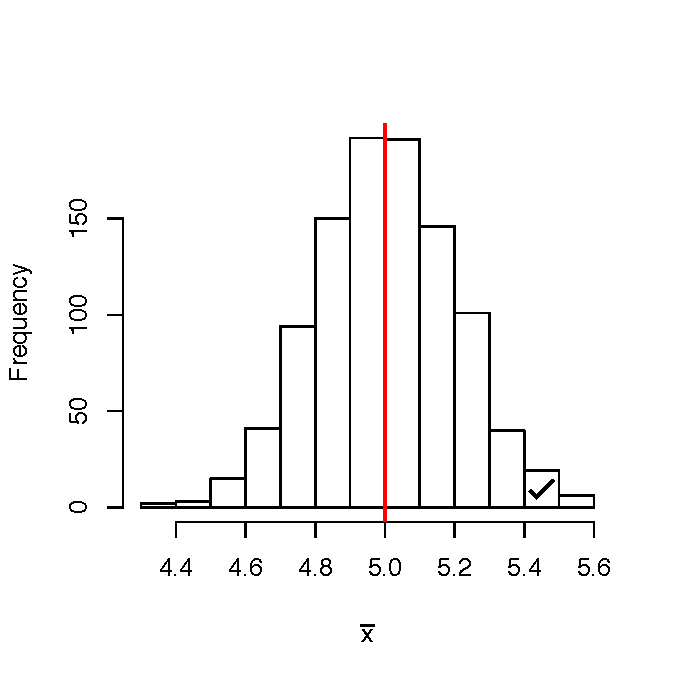
\includegraphics{figure/lec12-001}
\end{center}
\end{frame}
%-------------------------------------------------------------------------------


%------------------------------------------------------------------------------
\begin{frame}[fragile]
\frametitle{Sampling Distributions}

%
% Comment this
%
%\blue{Definition 2}: the \blue{sampling distribution} is the distribution of point estimates based on samples of fixed size $n$.  
%
%\pause \vspace{0.5cm}
%
%Every instance of a point estimate can be thought of as a draw from the sampling distribution.
%
%\pause \vspace{0.5cm}
%
%If the sampling is \blue{representative} (unbiased) then the sampling distribution will be centered around the true population parameter (in our case $\mu$).  

\end{frame}
%------------------------------------------------------------------------------


%------------------------------------------------------------------------------
\begin{frame}[fragile]
\frametitle{Sampling Distributions}

%
% Comment this
%
We can define the sampling distributions for \blue{any} point estimate, not just $\xbar$:
\pause \begin{itemize}
\item $s$
\item the sample median
\item etc.
\end{itemize}

\pause We will only focus on sample means, including the sample proportion $\widehat{p}$.

\end{frame}
%------------------------------------------------------------------------------


%-------------------------------------------------------------------------------
\begin{frame}[fragile]
\frametitle{Measure of Spread}
What about spread?  $[4.6, 5.4]$ contains roughly 95\% of the data.

\begin{columns}[c]
\column{.35\textwidth}
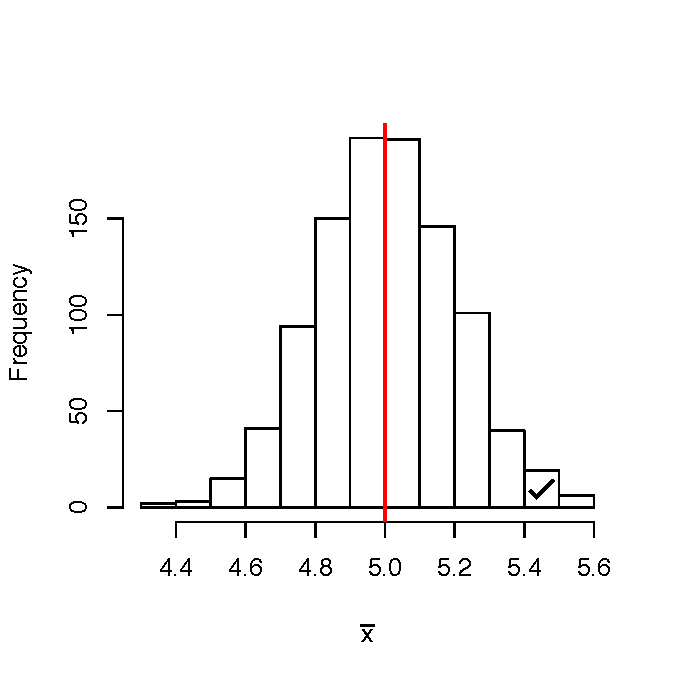
\includegraphics[width=5cm]{figure/lec12-001}
%\pause\column{.65\textwidth}
%\begin{eqnarray*}
%&& [\mu - 2 SD, \mu + 2SD] = [4.6, 5.4]\\
%&\Rightarrow& \mbox{length of interval is } 4SD = 5.4-4.6\\
%&\Rightarrow& SD = 0.2
%\end{eqnarray*}
\end{columns}




\end{frame}
%-------------------------------------------------------------------------------


%------------------------------------------------------------------------------
\begin{frame}[fragile]
\frametitle{Standard Errors}

%
% Comment this
%
%\blue{Definition 3}: The \blue{standard error} is the standard deviation of the sampling distribution of a point estimate.  
%
%\pause \vspace{0.5cm}
%
%It describes the uncertainty/variability associated with the point estimate.  In other words, the ``typical'' error.  
%
%\pause \vspace{0.5cm}
%
%\blue{Confusing}:  the \blue{standard error} is a specific kind of standard deviation.

\end{frame}
%------------------------------------------------------------------------------



%------------------------------------------------------------------------------
\begin{frame}[fragile]
\frametitle{Standard Error of $\xbar$}

%
% Comment this
%
%Given $n$ \blue{independent} observations from a population with standard deviation $\sigma$, the \blue{standard error of the sample mean} is
%\[
%SE = \frac{\sigma}{\sqrt{n}}
%\]
%
%\pause \blue{Rule of thumb for independence}:  You need a simple random sample consisting of less than 10\% of the population.  
%
%\vspace{0.5cm}
%\blue{Notice}: $\sqrt{n}$ in the denominator: as $n$ increases, SE decreases! This is why sample size matters.

\end{frame}
%------------------------------------------------------------------------------


%------------------------------------------------------------------------------
\begin{frame}[fragile]
\frametitle{Back to Histogram}
Samples were of size $n=100$ with $\sigma=2$.  We estimated that the SD was 0.2. 
\begin{center}
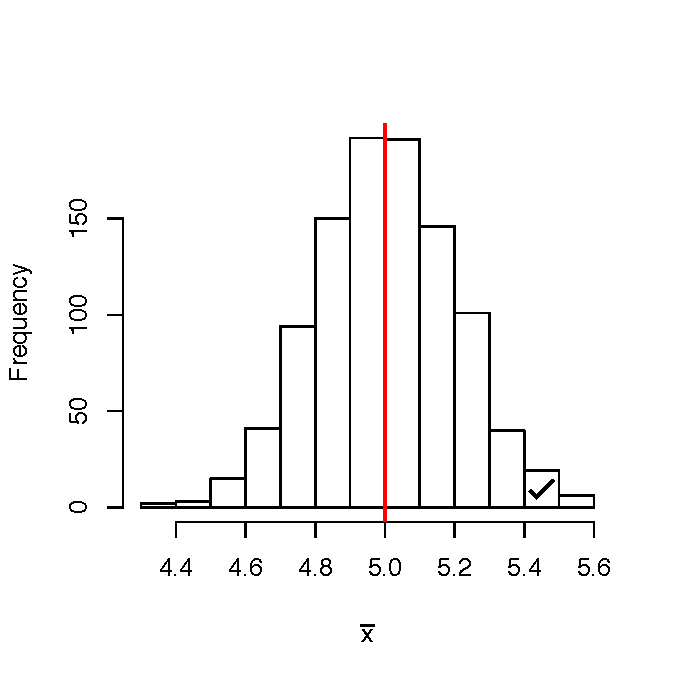
\includegraphics[width=0.5\textwidth]{figure/lec12-001}
\end{center}

\pause Using the formula:
\[
SE = \frac{\sigma}{\sqrt{n}} = \frac{2}{\sqrt{100}} = \frac{2}{10} = 0.2
\]

\end{frame}
%------------------------------------------------------------------------------




%pdf("./5.2 Variability in Estimates/compare.pdf", height=4.5, width=2*4.5)
%par(mfrow=c(1,2))
%xbar <- rep(0,1000)
%for(i in 1:1000)
%  xbar[i] <- mean(rnorm(n=100,mean=5,sd=2))
%hist(xbar, xlab=expression(bar(x)), main="", xlim=c(4.25, 5.75))
%title("n = 100")
%abline(v=5,col="red",lwd=2)
%
%xbar <- rep(0,1000)
%for(i in 1:1000)
%  xbar[i] <- mean(rnorm(n=1000,mean=5,sd=2))
%hist(xbar, xlab=expression(bar(x)), main="", xlim=c(4.25, 5.75))
%title("n = 1000")
%abline(v=5,col="red",lwd=2)
%dev.off()
%------------------------------------------------------------------------------
\begin{frame}[fragile]
\frametitle{Standard Error of the Sample Mean $\xbar$}
Compare 1000 instances of $\xbar$ when 
\begin{itemize}
\pause \item $n=100$. $SE = \frac{2}{\sqrt{100}} = 0.2$
\pause \item $n=1000$. $SE = \frac{2}{\sqrt{1000}} = 0.0632$.  \blue{Smaller}!
\end{itemize}

\begin{center}
\pause 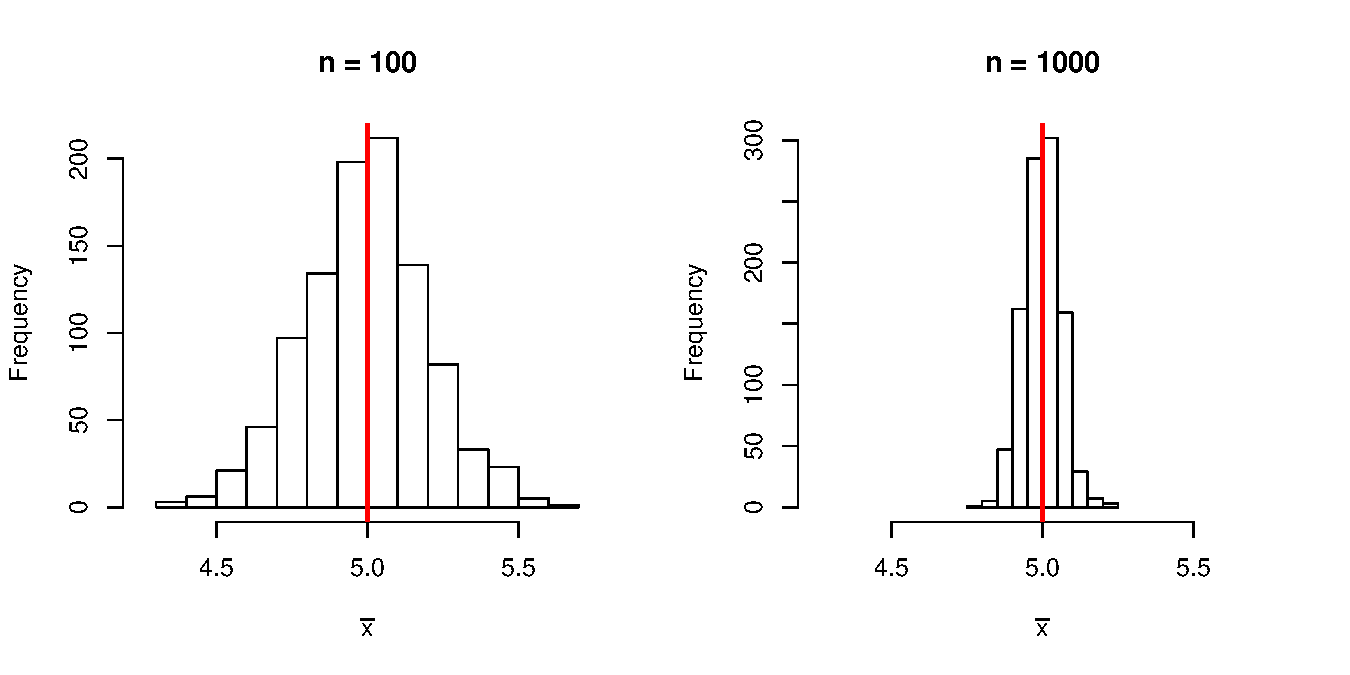
\includegraphics[width=0.8\textwidth]{figure/compare}
\end{center}
\pause Both are ``accurate'', but estimates on the right are ``more precise.''

\end{frame}
%------------------------------------------------------------------------------


%------------------------------------------------------------------------------
\begin{frame}[fragile]
\frametitle{Repeated Sampling}
%
% Comment this
%
%\blue{Popular question}:  Why would you take 1000 different samples of size $n$? 
%
%\vspace{0.5cm}
%
%\pause\blue{Answer}: No, in practice you would \blue{not} do this:  you do this only \blue{once} for the largest $n$ possible.  
%
%\vspace{0.5cm}
%
%\pause The 1000 instances of $\xbar$ is a rhetorical exercise to illustrate the random behavior of $\xbar$'s.  

\end{frame}
%------------------------------------------------------------------------------



%------------------------------------------------------------------------------
\begin{frame}[fragile]
\frametitle{Standard Error of the Sample Mean}

%
% Comment this
%
%In this example we knew $\sigma$; typically we won't.  
%
%\pause \vspace{0.25cm}
%
%However, when
%\begin{itemize}
%\item $n \geq 30$
%\pause \item the distribution of the population is \blue{not} strongly skewed
%\end{itemize}
%
%\vspace{0.25cm}
%
%\pause we can use the point estimate of $\sigma$.  i.e. plug in $s$ in place of $\sigma$:
%\[
%SE = \frac{s}{\sqrt{n}}
%\]

\end{frame}
%------------------------------------------------------------------------------


%%------------------------------------------------------------------------------
%\begin{frame}[fragile]
%\frametitle{Example}
%
%Say in you take a simple random sample of 100 runners in a race and you are interested in their ages:
%\begin{itemize}
%\item $\xbar = 35.05$
%\item $s=8.97$
%\end{itemize}
%
%\vspace{0.5cm}
%
%\pause Assuming that the 100 runners consist of less than 10\% of the population, the standard error of $\xbar$ is 
%\[
%SE = \frac{s}{\sqrt{100}} = \frac{8.97}{10} = 0.897
%\]
%
%
%\end{frame}
%%------------------------------------------------------------------------------


%------------------------------------------------------------------------------
\begin{frame}[fragile]
\frametitle{Population Distribution vs Sampling Distribution}


\end{frame}
%------------------------------------------------------------------------------


%------------------------------------------------------------------------------
\begin{frame}[fragile]
\frametitle{Recap}

\begin{itemize}
\item \blue{Point estimates} are based on a sample $x_1, \ldots, x_n$ and are used to estimate population parameters.
\pause \item The \blue{sampling distribution} characterizes the (random) behavior of point estimates.  
\pause \item The standard deviation of a sampling distribution is the \blue{standard error}: it quantifies the uncertainty/variability of point estimates.  
\end{itemize}

\end{frame}
%------------------------------------------------------------------------------


%------------------------------------------------------------------------------
\begin{frame}[fragile]
\frametitle{Next Time}

\begin{itemize}
\item Confidence Intervals
\item When quoting survey results, what does: ``the results of this survey are estimated to be accurate within 3.1 percentage points, 19 times out of 20'' mean?  
\item \blue{Big One}: Central Limit Theorem
\end{itemize}

\end{frame}
%------------------------------------------------------------------------------


\end{document}


